% Graphic for TeX using PGF
% Title: D:\Dokumente\GitHub\Bachelorarbeit\Arbeitstagebuch\src\29.06.2017-GeoNonTerm-classdiagram.dia
% Creator: Dia v0.97.2
% CreationDate: Fri Jun 30 11:40:19 2017
% For: Timo Bergerbusch
% \usepackage{tikz}
% The following commands are not supported in PSTricks at present
% We define them conditionally, so when they are implemented,
% this pgf file will use them.
\ifx\du\undefined
  \newlength{\du}
\fi
\setlength{\du}{15\unitlength}
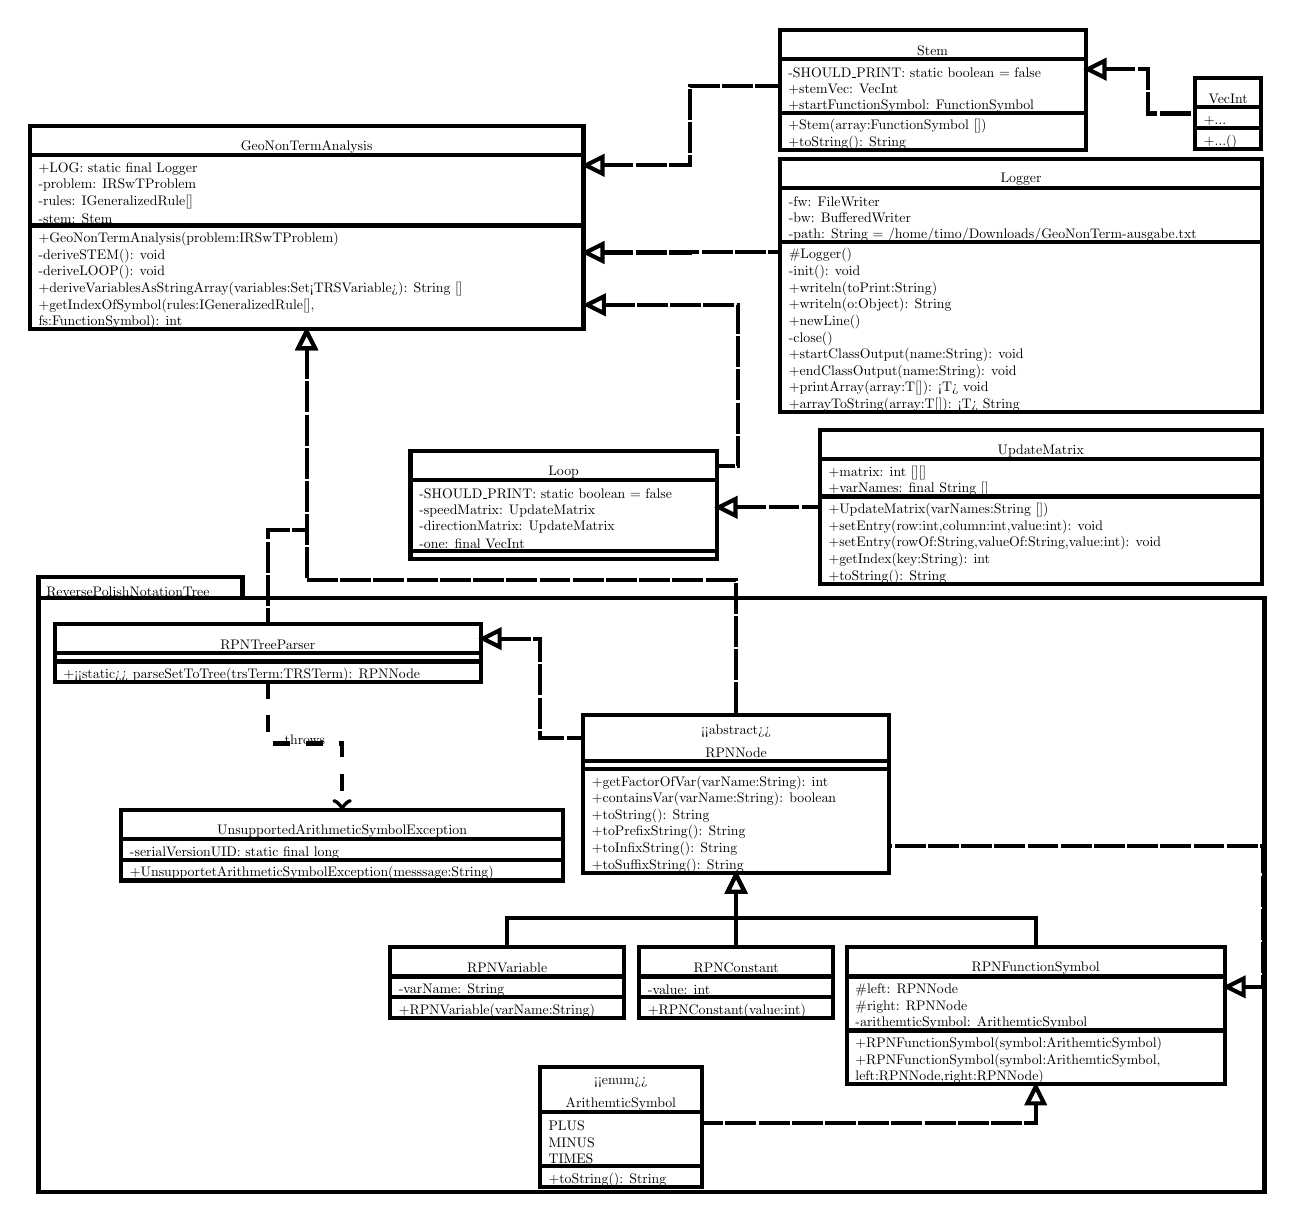
\begin{tikzpicture}[scale=0.5, every node/.style={scale=0.5}]
\pgftransformxscale{1.000000}
\pgftransformyscale{-1.000000}
\definecolor{dialinecolor}{rgb}{0.000000, 0.000000, 0.000000}
\pgfsetstrokecolor{dialinecolor}
\definecolor{dialinecolor}{rgb}{1.000000, 1.000000, 1.000000}
\pgfsetfillcolor{dialinecolor}
\pgfsetlinewidth{0.100000\du}
\pgfsetdash{}{0pt}
\definecolor{dialinecolor}{rgb}{1.000000, 1.000000, 1.000000}
\pgfsetfillcolor{dialinecolor}
\fill (-0.400221\du,9.418764\du)--(-0.400221\du,10.818764\du)--(26.279779\du,10.818764\du)--(26.279779\du,9.418764\du)--cycle;
\definecolor{dialinecolor}{rgb}{0.000000, 0.000000, 0.000000}
\pgfsetstrokecolor{dialinecolor}
\draw (-0.400221\du,9.418764\du)--(-0.400221\du,10.818764\du)--(26.279779\du,10.818764\du)--(26.279779\du,9.418764\du)--cycle;
% setfont left to latex
\definecolor{dialinecolor}{rgb}{0.000000, 0.000000, 0.000000}
\pgfsetstrokecolor{dialinecolor}
\node at (12.939779\du,10.418764\du){GeoNonTermAnalysis};
\definecolor{dialinecolor}{rgb}{1.000000, 1.000000, 1.000000}
\pgfsetfillcolor{dialinecolor}
\fill (-0.400221\du,10.818764\du)--(-0.400221\du,14.218764\du)--(26.279779\du,14.218764\du)--(26.279779\du,10.818764\du)--cycle;
\definecolor{dialinecolor}{rgb}{0.000000, 0.000000, 0.000000}
\pgfsetstrokecolor{dialinecolor}
\draw (-0.400221\du,10.818764\du)--(-0.400221\du,14.218764\du)--(26.279779\du,14.218764\du)--(26.279779\du,10.818764\du)--cycle;
% setfont left to latex
\definecolor{dialinecolor}{rgb}{0.000000, 0.000000, 0.000000}
\pgfsetstrokecolor{dialinecolor}
\node[anchor=west] at (-0.250221\du,11.478764\du){+LOG: static final Logger};
% setfont left to latex
\definecolor{dialinecolor}{rgb}{0.000000, 0.000000, 0.000000}
\pgfsetstrokecolor{dialinecolor}
\node[anchor=west] at (-0.250221\du,12.278764\du){-problem: IRSwTProblem};
% setfont left to latex
\definecolor{dialinecolor}{rgb}{0.000000, 0.000000, 0.000000}
\pgfsetstrokecolor{dialinecolor}
\node[anchor=west] at (-0.250221\du,13.078764\du){-rules: IGeneralizedRule\ensuremath{[}\ensuremath{]}};
% setfont left to latex
\definecolor{dialinecolor}{rgb}{0.000000, 0.000000, 0.000000}
\pgfsetstrokecolor{dialinecolor}
\node[anchor=west] at (-0.250221\du,13.878764\du){-stem: Stem};
\definecolor{dialinecolor}{rgb}{1.000000, 1.000000, 1.000000}
\pgfsetfillcolor{dialinecolor}
\fill (-0.400221\du,14.218764\du)--(-0.400221\du,19.218764\du)--(26.279779\du,19.218764\du)--(26.279779\du,14.218764\du)--cycle;
\definecolor{dialinecolor}{rgb}{0.000000, 0.000000, 0.000000}
\pgfsetstrokecolor{dialinecolor}
\draw (-0.400221\du,14.218764\du)--(-0.400221\du,19.218764\du)--(26.279779\du,19.218764\du)--(26.279779\du,14.218764\du)--cycle;
% setfont left to latex
\definecolor{dialinecolor}{rgb}{0.000000, 0.000000, 0.000000}
\pgfsetstrokecolor{dialinecolor}
\node[anchor=west] at (-0.250221\du,14.878764\du){+GeoNonTermAnalysis(problem:IRSwTProblem)};
% setfont left to latex
\definecolor{dialinecolor}{rgb}{0.000000, 0.000000, 0.000000}
\pgfsetstrokecolor{dialinecolor}
\node[anchor=west] at (-0.250221\du,15.678764\du){-deriveSTEM(): void};
% setfont left to latex
\definecolor{dialinecolor}{rgb}{0.000000, 0.000000, 0.000000}
\pgfsetstrokecolor{dialinecolor}
\node[anchor=west] at (-0.250221\du,16.478764\du){-deriveLOOP(): void};
% setfont left to latex
\definecolor{dialinecolor}{rgb}{0.000000, 0.000000, 0.000000}
\pgfsetstrokecolor{dialinecolor}
\node[anchor=west] at (-0.250221\du,17.278764\du){+deriveVariablesAsStringArray(variables:Set<TRSVariable>): String \ensuremath{[}\ensuremath{]}};
% setfont left to latex
\definecolor{dialinecolor}{rgb}{0.000000, 0.000000, 0.000000}
\pgfsetstrokecolor{dialinecolor}
\node[anchor=west] at (-0.250221\du,18.078764\du){+getIndexOfSymbol(rules:IGeneralizedRule\ensuremath{[}\ensuremath{]},};
\definecolor{dialinecolor}{rgb}{0.000000, 0.000000, 0.000000}
\pgfsetstrokecolor{dialinecolor}
\node[anchor=west] at (-0.250221\du,18.878764\du){                  fs:FunctionSymbol): int};
\pgfsetlinewidth{0.100000\du}
\pgfsetdash{}{0pt}
\definecolor{dialinecolor}{rgb}{1.000000, 1.000000, 1.000000}
\pgfsetfillcolor{dialinecolor}
\fill (35.727317\du,4.787296\du)--(35.727317\du,6.187296\du)--(50.472317\du,6.187296\du)--(50.472317\du,4.787296\du)--cycle;
\definecolor{dialinecolor}{rgb}{0.000000, 0.000000, 0.000000}
\pgfsetstrokecolor{dialinecolor}
\draw (35.727317\du,4.787296\du)--(35.727317\du,6.187296\du)--(50.472317\du,6.187296\du)--(50.472317\du,4.787296\du)--cycle;
% setfont left to latex
\definecolor{dialinecolor}{rgb}{0.000000, 0.000000, 0.000000}
\pgfsetstrokecolor{dialinecolor}
\node at (43.099817\du,5.787296\du){Stem};
\definecolor{dialinecolor}{rgb}{1.000000, 1.000000, 1.000000}
\pgfsetfillcolor{dialinecolor}
\fill (35.727317\du,6.187296\du)--(35.727317\du,8.787296\du)--(50.472317\du,8.787296\du)--(50.472317\du,6.187296\du)--cycle;
\definecolor{dialinecolor}{rgb}{0.000000, 0.000000, 0.000000}
\pgfsetstrokecolor{dialinecolor}
\draw (35.727317\du,6.187296\du)--(35.727317\du,8.787296\du)--(50.472317\du,8.787296\du)--(50.472317\du,6.187296\du)--cycle;
% setfont left to latex
\definecolor{dialinecolor}{rgb}{0.000000, 0.000000, 0.000000}
\pgfsetstrokecolor{dialinecolor}
\node[anchor=west] at (35.877317\du,6.847296\du){-SHOULD\_PRINT: static boolean = false};
% setfont left to latex
\definecolor{dialinecolor}{rgb}{0.000000, 0.000000, 0.000000}
\pgfsetstrokecolor{dialinecolor}
\node[anchor=west] at (35.877317\du,7.647296\du){+stemVec: VecInt};
% setfont left to latex
\definecolor{dialinecolor}{rgb}{0.000000, 0.000000, 0.000000}
\pgfsetstrokecolor{dialinecolor}
\node[anchor=west] at (35.877317\du,8.447296\du){+startFunctionSymbol: FunctionSymbol};
\definecolor{dialinecolor}{rgb}{1.000000, 1.000000, 1.000000}
\pgfsetfillcolor{dialinecolor}
\fill (35.727317\du,8.787296\du)--(35.727317\du,10.587296\du)--(50.472317\du,10.587296\du)--(50.472317\du,8.787296\du)--cycle;
\definecolor{dialinecolor}{rgb}{0.000000, 0.000000, 0.000000}
\pgfsetstrokecolor{dialinecolor}
\draw (35.727317\du,8.787296\du)--(35.727317\du,10.587296\du)--(50.472317\du,10.587296\du)--(50.472317\du,8.787296\du)--cycle;
% setfont left to latex
\definecolor{dialinecolor}{rgb}{0.000000, 0.000000, 0.000000}
\pgfsetstrokecolor{dialinecolor}
\node[anchor=west] at (35.877317\du,9.447296\du){+Stem(array:FunctionSymbol \ensuremath{[}\ensuremath{]})};
% setfont left to latex
\definecolor{dialinecolor}{rgb}{0.000000, 0.000000, 0.000000}
\pgfsetstrokecolor{dialinecolor}
\node[anchor=west] at (35.877317\du,10.247296\du){+toString(): String};
\pgfsetlinewidth{0.100000\du}
\pgfsetdash{}{0pt}
\definecolor{dialinecolor}{rgb}{1.000000, 1.000000, 1.000000}
\pgfsetfillcolor{dialinecolor}
\fill (55.750533\du,7.125555\du)--(55.750533\du,8.525555\du)--(58.933033\du,8.525555\du)--(58.933033\du,7.125555\du)--cycle;
\definecolor{dialinecolor}{rgb}{0.000000, 0.000000, 0.000000}
\pgfsetstrokecolor{dialinecolor}
\draw (55.750533\du,7.125555\du)--(55.750533\du,8.525555\du)--(58.933033\du,8.525555\du)--(58.933033\du,7.125555\du)--cycle;
% setfont left to latex
\definecolor{dialinecolor}{rgb}{0.000000, 0.000000, 0.000000}
\pgfsetstrokecolor{dialinecolor}
\node at (57.341783\du,8.125555\du){VecInt};
\definecolor{dialinecolor}{rgb}{1.000000, 1.000000, 1.000000}
\pgfsetfillcolor{dialinecolor}
\fill (55.750533\du,8.525555\du)--(55.750533\du,9.525555\du)--(58.933033\du,9.525555\du)--(58.933033\du,8.525555\du)--cycle;
\definecolor{dialinecolor}{rgb}{0.000000, 0.000000, 0.000000}
\pgfsetstrokecolor{dialinecolor}
\draw (55.750533\du,8.525555\du)--(55.750533\du,9.525555\du)--(58.933033\du,9.525555\du)--(58.933033\du,8.525555\du)--cycle;
% setfont left to latex
\definecolor{dialinecolor}{rgb}{0.000000, 0.000000, 0.000000}
\pgfsetstrokecolor{dialinecolor}
\node[anchor=west] at (55.900533\du,9.185555\du){+...};
\definecolor{dialinecolor}{rgb}{1.000000, 1.000000, 1.000000}
\pgfsetfillcolor{dialinecolor}
\fill (55.750533\du,9.525555\du)--(55.750533\du,10.525555\du)--(58.933033\du,10.525555\du)--(58.933033\du,9.525555\du)--cycle;
\definecolor{dialinecolor}{rgb}{0.000000, 0.000000, 0.000000}
\pgfsetstrokecolor{dialinecolor}
\draw (55.750533\du,9.525555\du)--(55.750533\du,10.525555\du)--(58.933033\du,10.525555\du)--(58.933033\du,9.525555\du)--cycle;
% setfont left to latex
\definecolor{dialinecolor}{rgb}{0.000000, 0.000000, 0.000000}
\pgfsetstrokecolor{dialinecolor}
\node[anchor=west] at (55.900533\du,10.185555\du){+...()};
\pgfsetlinewidth{0.100000\du}
\pgfsetdash{{1.000000\du}{1.000000\du}}{0\du}
\pgfsetdash{{0.400000\du}{0.400000\du}}{0\du}
\pgfsetmiterjoin
\pgfsetbuttcap
{
\definecolor{dialinecolor}{rgb}{0.000000, 0.000000, 0.000000}
\pgfsetfillcolor{dialinecolor}
% was here!!!
\definecolor{dialinecolor}{rgb}{0.000000, 0.000000, 0.000000}
\pgfsetstrokecolor{dialinecolor}
\draw (26.279779\du,11.318764\du)--(31.403548\du,11.318764\du)--(31.403548\du,7.487296\du)--(35.727317\du,7.487296\du);
}
\definecolor{dialinecolor}{rgb}{0.000000, 0.000000, 0.000000}
\pgfsetstrokecolor{dialinecolor}
\draw (27.191583\du,11.318764\du)--(31.403548\du,11.318764\du)--(31.403548\du,7.487296\du)--(35.727317\du,7.487296\du);
\pgfsetmiterjoin
\definecolor{dialinecolor}{rgb}{1.000000, 1.000000, 1.000000}
\pgfsetfillcolor{dialinecolor}
\fill (27.191583\du,10.918764\du)--(26.391583\du,11.318764\du)--(27.191583\du,11.718764\du)--cycle;
\pgfsetlinewidth{0.100000\du}
\pgfsetdash{}{0pt}
\pgfsetmiterjoin
\definecolor{dialinecolor}{rgb}{0.000000, 0.000000, 0.000000}
\pgfsetstrokecolor{dialinecolor}
\draw (27.191583\du,10.918764\du)--(26.391583\du,11.318764\du)--(27.191583\du,11.718764\du)--cycle;
% setfont left to latex
\pgfsetlinewidth{0.100000\du}
\pgfsetdash{}{0pt}
\definecolor{dialinecolor}{rgb}{1.000000, 1.000000, 1.000000}
\pgfsetfillcolor{dialinecolor}
\fill (35.751336\du,11.005288\du)--(35.751336\du,12.405288\du)--(58.966336\du,12.405288\du)--(58.966336\du,11.005288\du)--cycle;
\definecolor{dialinecolor}{rgb}{0.000000, 0.000000, 0.000000}
\pgfsetstrokecolor{dialinecolor}
\draw (35.751336\du,11.005288\du)--(35.751336\du,12.405288\du)--(58.966336\du,12.405288\du)--(58.966336\du,11.005288\du)--cycle;
% setfont left to latex
\definecolor{dialinecolor}{rgb}{0.000000, 0.000000, 0.000000}
\pgfsetstrokecolor{dialinecolor}
\node at (47.358836\du,12.005288\du){Logger};
\definecolor{dialinecolor}{rgb}{1.000000, 1.000000, 1.000000}
\pgfsetfillcolor{dialinecolor}
\fill (35.751336\du,12.405288\du)--(35.751336\du,15.005288\du)--(58.966336\du,15.005288\du)--(58.966336\du,12.405288\du)--cycle;
\definecolor{dialinecolor}{rgb}{0.000000, 0.000000, 0.000000}
\pgfsetstrokecolor{dialinecolor}
\draw (35.751336\du,12.405288\du)--(35.751336\du,15.005288\du)--(58.966336\du,15.005288\du)--(58.966336\du,12.405288\du)--cycle;
% setfont left to latex
\definecolor{dialinecolor}{rgb}{0.000000, 0.000000, 0.000000}
\pgfsetstrokecolor{dialinecolor}
\node[anchor=west] at (35.901336\du,13.065288\du){-fw: FileWriter};
% setfont left to latex
\definecolor{dialinecolor}{rgb}{0.000000, 0.000000, 0.000000}
\pgfsetstrokecolor{dialinecolor}
\node[anchor=west] at (35.901336\du,13.865288\du){-bw: BufferedWriter};
% setfont left to latex
\definecolor{dialinecolor}{rgb}{0.000000, 0.000000, 0.000000}
\pgfsetstrokecolor{dialinecolor}
\node[anchor=west] at (35.901336\du,14.665288\du){-path: String = /home/timo/Downloads/GeoNonTerm-ausgabe.txt};
\definecolor{dialinecolor}{rgb}{1.000000, 1.000000, 1.000000}
\pgfsetfillcolor{dialinecolor}
\fill (35.751336\du,15.005288\du)--(35.751336\du,23.205288\du)--(58.966336\du,23.205288\du)--(58.966336\du,15.005288\du)--cycle;
\definecolor{dialinecolor}{rgb}{0.000000, 0.000000, 0.000000}
\pgfsetstrokecolor{dialinecolor}
\draw (35.751336\du,15.005288\du)--(35.751336\du,23.205288\du)--(58.966336\du,23.205288\du)--(58.966336\du,15.005288\du)--cycle;
% setfont left to latex
\definecolor{dialinecolor}{rgb}{0.000000, 0.000000, 0.000000}
\pgfsetstrokecolor{dialinecolor}
\node[anchor=west] at (35.901336\du,15.665288\du){\#Logger()};
% setfont left to latex
\definecolor{dialinecolor}{rgb}{0.000000, 0.000000, 0.000000}
\pgfsetstrokecolor{dialinecolor}
\node[anchor=west] at (35.901336\du,16.465288\du){-init(): void};
% setfont left to latex
\definecolor{dialinecolor}{rgb}{0.000000, 0.000000, 0.000000}
\pgfsetstrokecolor{dialinecolor}
\node[anchor=west] at (35.901336\du,17.265288\du){+writeln(toPrint:String)};
% setfont left to latex
\definecolor{dialinecolor}{rgb}{0.000000, 0.000000, 0.000000}
\pgfsetstrokecolor{dialinecolor}
\node[anchor=west] at (35.901336\du,18.065288\du){+writeln(o:Object): String};
% setfont left to latex
\definecolor{dialinecolor}{rgb}{0.000000, 0.000000, 0.000000}
\pgfsetstrokecolor{dialinecolor}
\node[anchor=west] at (35.901336\du,18.865288\du){+newLine()};
% setfont left to latex
\definecolor{dialinecolor}{rgb}{0.000000, 0.000000, 0.000000}
\pgfsetstrokecolor{dialinecolor}
\node[anchor=west] at (35.901336\du,19.665288\du){-close()};
% setfont left to latex
\definecolor{dialinecolor}{rgb}{0.000000, 0.000000, 0.000000}
\pgfsetstrokecolor{dialinecolor}
\node[anchor=west] at (35.901336\du,20.465288\du){+startClassOutput(name:String): void};
% setfont left to latex
\definecolor{dialinecolor}{rgb}{0.000000, 0.000000, 0.000000}
\pgfsetstrokecolor{dialinecolor}
\node[anchor=west] at (35.901336\du,21.265288\du){+endClassOutput(name:String): void};
% setfont left to latex
\definecolor{dialinecolor}{rgb}{0.000000, 0.000000, 0.000000}
\pgfsetstrokecolor{dialinecolor}
\node[anchor=west] at (35.901336\du,22.065288\du){+printArray(array:T\ensuremath{[}\ensuremath{]}): <T> void};
% setfont left to latex
\definecolor{dialinecolor}{rgb}{0.000000, 0.000000, 0.000000}
\pgfsetstrokecolor{dialinecolor}
\node[anchor=west] at (35.901336\du,22.865288\du){+arrayToString(array:T\ensuremath{[}\ensuremath{]}): <T> String};
\pgfsetlinewidth{0.100000\du}
\pgfsetdash{{0.400000\du}{0.400000\du}}{0\du}
\pgfsetdash{{0.400000\du}{0.400000\du}}{0\du}
\pgfsetmiterjoin
\pgfsetbuttcap
{
\definecolor{dialinecolor}{rgb}{0.000000, 0.000000, 0.000000}
\pgfsetfillcolor{dialinecolor}
% was here!!!
\definecolor{dialinecolor}{rgb}{0.000000, 0.000000, 0.000000}
\pgfsetstrokecolor{dialinecolor}
\draw (26.279779\du,15.518764\du)--(31.415558\du,15.518764\du)--(31.415558\du,15.505288\du)--(35.751336\du,15.505288\du);
}
\definecolor{dialinecolor}{rgb}{0.000000, 0.000000, 0.000000}
\pgfsetstrokecolor{dialinecolor}
\draw (27.191583\du,15.518764\du)--(31.415558\du,15.518764\du)--(31.415558\du,15.505288\du)--(35.751336\du,15.505288\du);
\pgfsetmiterjoin
\definecolor{dialinecolor}{rgb}{1.000000, 1.000000, 1.000000}
\pgfsetfillcolor{dialinecolor}
\fill (27.191583\du,15.118764\du)--(26.391583\du,15.518764\du)--(27.191583\du,15.918764\du)--cycle;
\pgfsetlinewidth{0.100000\du}
\pgfsetdash{}{0pt}
\pgfsetmiterjoin
\definecolor{dialinecolor}{rgb}{0.000000, 0.000000, 0.000000}
\pgfsetstrokecolor{dialinecolor}
\draw (27.191583\du,15.118764\du)--(26.391583\du,15.518764\du)--(27.191583\du,15.918764\du)--cycle;
% setfont left to latex
\pgfsetlinewidth{0.100000\du}
\pgfsetdash{{0.400000\du}{0.400000\du}}{0\du}
\pgfsetdash{{0.400000\du}{0.400000\du}}{0\du}
\pgfsetmiterjoin
\pgfsetbuttcap
{
\definecolor{dialinecolor}{rgb}{0.000000, 0.000000, 0.000000}
\pgfsetfillcolor{dialinecolor}
% was here!!!
\definecolor{dialinecolor}{rgb}{0.000000, 0.000000, 0.000000}
\pgfsetstrokecolor{dialinecolor}
\draw (50.472317\du,6.687296\du)--(53.486224\du,6.687296\du)--(53.486224\du,8.825555\du)--(55.700132\du,8.825555\du);
}
\definecolor{dialinecolor}{rgb}{0.000000, 0.000000, 0.000000}
\pgfsetstrokecolor{dialinecolor}
\draw (51.384120\du,6.687296\du)--(53.486224\du,6.687296\du)--(53.486224\du,8.825555\du)--(55.700132\du,8.825555\du);
\pgfsetmiterjoin
\definecolor{dialinecolor}{rgb}{1.000000, 1.000000, 1.000000}
\pgfsetfillcolor{dialinecolor}
\fill (51.384120\du,6.287296\du)--(50.584120\du,6.687296\du)--(51.384120\du,7.087296\du)--cycle;
\pgfsetlinewidth{0.100000\du}
\pgfsetdash{}{0pt}
\pgfsetmiterjoin
\definecolor{dialinecolor}{rgb}{0.000000, 0.000000, 0.000000}
\pgfsetstrokecolor{dialinecolor}
\draw (51.384120\du,6.287296\du)--(50.584120\du,6.687296\du)--(51.384120\du,7.087296\du)--cycle;
% setfont left to latex
\pgfsetlinewidth{0.100000\du}
\pgfsetdash{}{0pt}
\definecolor{dialinecolor}{rgb}{1.000000, 1.000000, 1.000000}
\pgfsetfillcolor{dialinecolor}
\fill (17.947367\du,25.094337\du)--(17.947367\du,26.494337\du)--(32.692367\du,26.494337\du)--(32.692367\du,25.094337\du)--cycle;
\definecolor{dialinecolor}{rgb}{0.000000, 0.000000, 0.000000}
\pgfsetstrokecolor{dialinecolor}
\draw (17.947367\du,25.094337\du)--(17.947367\du,26.494337\du)--(32.692367\du,26.494337\du)--(32.692367\du,25.094337\du)--cycle;
% setfont left to latex
\definecolor{dialinecolor}{rgb}{0.000000, 0.000000, 0.000000}
\pgfsetstrokecolor{dialinecolor}
\node at (25.319867\du,26.094337\du){Loop};
\definecolor{dialinecolor}{rgb}{1.000000, 1.000000, 1.000000}
\pgfsetfillcolor{dialinecolor}
\fill (17.947367\du,26.494337\du)--(17.947367\du,29.894337\du)--(32.692367\du,29.894337\du)--(32.692367\du,26.494337\du)--cycle;
\definecolor{dialinecolor}{rgb}{0.000000, 0.000000, 0.000000}
\pgfsetstrokecolor{dialinecolor}
\draw (17.947367\du,26.494337\du)--(17.947367\du,29.894337\du)--(32.692367\du,29.894337\du)--(32.692367\du,26.494337\du)--cycle;
% setfont left to latex
\definecolor{dialinecolor}{rgb}{0.000000, 0.000000, 0.000000}
\pgfsetstrokecolor{dialinecolor}
\node[anchor=west] at (18.097367\du,27.154337\du){-SHOULD\_PRINT: static boolean = false};
% setfont left to latex
\definecolor{dialinecolor}{rgb}{0.000000, 0.000000, 0.000000}
\pgfsetstrokecolor{dialinecolor}
\node[anchor=west] at (18.097367\du,27.954337\du){-speedMatrix: UpdateMatrix};
% setfont left to latex
\definecolor{dialinecolor}{rgb}{0.000000, 0.000000, 0.000000}
\pgfsetstrokecolor{dialinecolor}
\node[anchor=west] at (18.097367\du,28.754337\du){-directionMatrix: UpdateMatrix};
% setfont left to latex
\definecolor{dialinecolor}{rgb}{0.000000, 0.000000, 0.000000}
\pgfsetstrokecolor{dialinecolor}
\node[anchor=west] at (18.097367\du,29.554337\du){-one: final VecInt};
\definecolor{dialinecolor}{rgb}{1.000000, 1.000000, 1.000000}
\pgfsetfillcolor{dialinecolor}
\fill (17.947367\du,29.894337\du)--(17.947367\du,30.294337\du)--(32.692367\du,30.294337\du)--(32.692367\du,29.894337\du)--cycle;
\definecolor{dialinecolor}{rgb}{0.000000, 0.000000, 0.000000}
\pgfsetstrokecolor{dialinecolor}
\draw (17.947367\du,29.894337\du)--(17.947367\du,30.294337\du)--(32.692367\du,30.294337\du)--(32.692367\du,29.894337\du)--cycle;
\pgfsetlinewidth{0.100000\du}
\pgfsetdash{{0.400000\du}{0.400000\du}}{0\du}
\pgfsetdash{{0.400000\du}{0.400000\du}}{0\du}
\pgfsetmiterjoin
\pgfsetbuttcap
{
\definecolor{dialinecolor}{rgb}{0.000000, 0.000000, 0.000000}
\pgfsetfillcolor{dialinecolor}
% was here!!!
\definecolor{dialinecolor}{rgb}{0.000000, 0.000000, 0.000000}
\pgfsetstrokecolor{dialinecolor}
\draw (26.347212\du,18.039672\du)--(33.742367\du,18.039672\du)--(33.742367\du,25.794337\du)--(32.692367\du,25.794337\du);
}
\definecolor{dialinecolor}{rgb}{0.000000, 0.000000, 0.000000}
\pgfsetstrokecolor{dialinecolor}
\draw (27.259015\du,18.039672\du)--(33.742367\du,18.039672\du)--(33.742367\du,25.794337\du)--(32.692367\du,25.794337\du);
\pgfsetmiterjoin
\definecolor{dialinecolor}{rgb}{1.000000, 1.000000, 1.000000}
\pgfsetfillcolor{dialinecolor}
\fill (27.259015\du,17.639672\du)--(26.459015\du,18.039672\du)--(27.259015\du,18.439672\du)--cycle;
\pgfsetlinewidth{0.100000\du}
\pgfsetdash{}{0pt}
\pgfsetmiterjoin
\definecolor{dialinecolor}{rgb}{0.000000, 0.000000, 0.000000}
\pgfsetstrokecolor{dialinecolor}
\draw (27.259015\du,17.639672\du)--(26.459015\du,18.039672\du)--(27.259015\du,18.439672\du)--cycle;
% setfont left to latex
\pgfsetlinewidth{0.100000\du}
\pgfsetdash{}{0pt}
\definecolor{dialinecolor}{rgb}{1.000000, 1.000000, 1.000000}
\pgfsetfillcolor{dialinecolor}
\fill (37.664586\du,24.077161\du)--(37.664586\du,25.477161\du)--(58.954586\du,25.477161\du)--(58.954586\du,24.077161\du)--cycle;
\definecolor{dialinecolor}{rgb}{0.000000, 0.000000, 0.000000}
\pgfsetstrokecolor{dialinecolor}
\draw (37.664586\du,24.077161\du)--(37.664586\du,25.477161\du)--(58.954586\du,25.477161\du)--(58.954586\du,24.077161\du)--cycle;
% setfont left to latex
\definecolor{dialinecolor}{rgb}{0.000000, 0.000000, 0.000000}
\pgfsetstrokecolor{dialinecolor}
\node at (48.309586\du,25.077161\du){UpdateMatrix};
\definecolor{dialinecolor}{rgb}{1.000000, 1.000000, 1.000000}
\pgfsetfillcolor{dialinecolor}
\fill (37.664586\du,25.477161\du)--(37.664586\du,27.277161\du)--(58.954586\du,27.277161\du)--(58.954586\du,25.477161\du)--cycle;
\definecolor{dialinecolor}{rgb}{0.000000, 0.000000, 0.000000}
\pgfsetstrokecolor{dialinecolor}
\draw (37.664586\du,25.477161\du)--(37.664586\du,27.277161\du)--(58.954586\du,27.277161\du)--(58.954586\du,25.477161\du)--cycle;
% setfont left to latex
\definecolor{dialinecolor}{rgb}{0.000000, 0.000000, 0.000000}
\pgfsetstrokecolor{dialinecolor}
\node[anchor=west] at (37.814586\du,26.137161\du){+matrix: int \ensuremath{[}\ensuremath{]}\ensuremath{[}\ensuremath{]}};
% setfont left to latex
\definecolor{dialinecolor}{rgb}{0.000000, 0.000000, 0.000000}
\pgfsetstrokecolor{dialinecolor}
\node[anchor=west] at (37.814586\du,26.937161\du){+varNames: final String \ensuremath{[}\ensuremath{]}};
\definecolor{dialinecolor}{rgb}{1.000000, 1.000000, 1.000000}
\pgfsetfillcolor{dialinecolor}
\fill (37.664586\du,27.277161\du)--(37.664586\du,31.477161\du)--(58.954586\du,31.477161\du)--(58.954586\du,27.277161\du)--cycle;
\definecolor{dialinecolor}{rgb}{0.000000, 0.000000, 0.000000}
\pgfsetstrokecolor{dialinecolor}
\draw (37.664586\du,27.277161\du)--(37.664586\du,31.477161\du)--(58.954586\du,31.477161\du)--(58.954586\du,27.277161\du)--cycle;
% setfont left to latex
\definecolor{dialinecolor}{rgb}{0.000000, 0.000000, 0.000000}
\pgfsetstrokecolor{dialinecolor}
\node[anchor=west] at (37.814586\du,27.937161\du){+UpdateMatrix(varNames:String \ensuremath{[}\ensuremath{]})};
% setfont left to latex
\definecolor{dialinecolor}{rgb}{0.000000, 0.000000, 0.000000}
\pgfsetstrokecolor{dialinecolor}
\node[anchor=west] at (37.814586\du,28.737161\du){+setEntry(row:int,column:int,value:int): void};
% setfont left to latex
\definecolor{dialinecolor}{rgb}{0.000000, 0.000000, 0.000000}
\pgfsetstrokecolor{dialinecolor}
\node[anchor=west] at (37.814586\du,29.537161\du){+setEntry(rowOf:String,valueOf:String,value:int): void};
% setfont left to latex
\definecolor{dialinecolor}{rgb}{0.000000, 0.000000, 0.000000}
\pgfsetstrokecolor{dialinecolor}
\node[anchor=west] at (37.814586\du,30.337161\du){+getIndex(key:String): int};
% setfont left to latex
\definecolor{dialinecolor}{rgb}{0.000000, 0.000000, 0.000000}
\pgfsetstrokecolor{dialinecolor}
\node[anchor=west] at (37.814586\du,31.137161\du){+toString(): String};
\pgfsetlinewidth{0.100000\du}
\pgfsetdash{{0.400000\du}{0.400000\du}}{0\du}
\pgfsetdash{{0.400000\du}{0.400000\du}}{0\du}
\pgfsetmiterjoin
\pgfsetbuttcap
{
\definecolor{dialinecolor}{rgb}{0.000000, 0.000000, 0.000000}
\pgfsetfillcolor{dialinecolor}
% was here!!!
\definecolor{dialinecolor}{rgb}{0.000000, 0.000000, 0.000000}
\pgfsetstrokecolor{dialinecolor}
\draw (32.692367\du,27.794337\du)--(35.578476\du,27.794337\du)--(35.578476\du,27.777161\du)--(37.664586\du,27.777161\du);
}
\definecolor{dialinecolor}{rgb}{0.000000, 0.000000, 0.000000}
\pgfsetstrokecolor{dialinecolor}
\draw (33.604170\du,27.794337\du)--(35.578476\du,27.794337\du)--(35.578476\du,27.777161\du)--(37.664586\du,27.777161\du);
\pgfsetmiterjoin
\definecolor{dialinecolor}{rgb}{1.000000, 1.000000, 1.000000}
\pgfsetfillcolor{dialinecolor}
\fill (33.604170\du,27.394337\du)--(32.804170\du,27.794337\du)--(33.604170\du,28.194337\du)--cycle;
\pgfsetlinewidth{0.100000\du}
\pgfsetdash{}{0pt}
\pgfsetmiterjoin
\definecolor{dialinecolor}{rgb}{0.000000, 0.000000, 0.000000}
\pgfsetstrokecolor{dialinecolor}
\draw (33.604170\du,27.394337\du)--(32.804170\du,27.794337\du)--(33.604170\du,28.194337\du)--cycle;
% setfont left to latex
\pgfsetlinewidth{0.100000\du}
\pgfsetdash{}{0pt}
\definecolor{dialinecolor}{rgb}{1.000000, 1.000000, 1.000000}
\pgfsetfillcolor{dialinecolor}
\fill (0.024881\du,32.161827\du)--(0.024881\du,60.777815\du)--(59.091812\du,60.777815\du)--(59.091812\du,32.161827\du)--cycle;
\definecolor{dialinecolor}{rgb}{0.000000, 0.000000, 0.000000}
\pgfsetstrokecolor{dialinecolor}
\draw (0.024881\du,32.161827\du)--(0.024881\du,60.777815\du)--(59.091812\du,60.777815\du)--(59.091812\du,32.161827\du)--cycle;
\definecolor{dialinecolor}{rgb}{1.000000, 1.000000, 1.000000}
\pgfsetfillcolor{dialinecolor}
\fill (0.024881\du,31.161827\du)--(0.024881\du,32.161827\du)--(9.849881\du,32.161827\du)--(9.849881\du,31.161827\du)--cycle;
\definecolor{dialinecolor}{rgb}{0.000000, 0.000000, 0.000000}
\pgfsetstrokecolor{dialinecolor}
\draw (0.024881\du,31.161827\du)--(0.024881\du,32.161827\du)--(9.849881\du,32.161827\du)--(9.849881\du,31.161827\du)--cycle;
% setfont left to latex
\definecolor{dialinecolor}{rgb}{0.000000, 0.000000, 0.000000}
\pgfsetstrokecolor{dialinecolor}
\node[anchor=west] at (0.124881\du,31.861827\du){ReversePolishNotationTree};
\pgfsetlinewidth{0.100000\du}
\pgfsetdash{}{0pt}
\definecolor{dialinecolor}{rgb}{1.000000, 1.000000, 1.000000}
\pgfsetfillcolor{dialinecolor}
\fill (26.261279\du,37.799990\du)--(26.261279\du,39.999990\du)--(41.006279\du,39.999990\du)--(41.006279\du,37.799990\du)--cycle;
\definecolor{dialinecolor}{rgb}{0.000000, 0.000000, 0.000000}
\pgfsetstrokecolor{dialinecolor}
\draw (26.261279\du,37.799990\du)--(26.261279\du,39.999990\du)--(41.006279\du,39.999990\du)--(41.006279\du,37.799990\du)--cycle;
% setfont left to latex
\definecolor{dialinecolor}{rgb}{0.000000, 0.000000, 0.000000}
\pgfsetstrokecolor{dialinecolor}
\node at (33.633779\du,38.559990\du){<<abstract>>};
% setfont left to latex
\definecolor{dialinecolor}{rgb}{0.000000, 0.000000, 0.000000}
\pgfsetstrokecolor{dialinecolor}
\node at (33.633779\du,39.599990\du){RPNNode};
\definecolor{dialinecolor}{rgb}{1.000000, 1.000000, 1.000000}
\pgfsetfillcolor{dialinecolor}
\fill (26.261279\du,39.999990\du)--(26.261279\du,40.399990\du)--(41.006279\du,40.399990\du)--(41.006279\du,39.999990\du)--cycle;
\definecolor{dialinecolor}{rgb}{0.000000, 0.000000, 0.000000}
\pgfsetstrokecolor{dialinecolor}
\draw (26.261279\du,39.999990\du)--(26.261279\du,40.399990\du)--(41.006279\du,40.399990\du)--(41.006279\du,39.999990\du)--cycle;
\definecolor{dialinecolor}{rgb}{1.000000, 1.000000, 1.000000}
\pgfsetfillcolor{dialinecolor}
\fill (26.261279\du,40.399990\du)--(26.261279\du,45.399990\du)--(41.006279\du,45.399990\du)--(41.006279\du,40.399990\du)--cycle;
\definecolor{dialinecolor}{rgb}{0.000000, 0.000000, 0.000000}
\pgfsetstrokecolor{dialinecolor}
\draw (26.261279\du,40.399990\du)--(26.261279\du,45.399990\du)--(41.006279\du,45.399990\du)--(41.006279\du,40.399990\du)--cycle;
% setfont left to latex
\definecolor{dialinecolor}{rgb}{0.000000, 0.000000, 0.000000}
\pgfsetstrokecolor{dialinecolor}
\node[anchor=west] at (26.411279\du,41.059990\du){+getFactorOfVar(varName:String): int};
% setfont left to latex
\definecolor{dialinecolor}{rgb}{0.000000, 0.000000, 0.000000}
\pgfsetstrokecolor{dialinecolor}
\node[anchor=west] at (26.411279\du,41.859990\du){+containsVar(varName:String): boolean};
% setfont left to latex
\definecolor{dialinecolor}{rgb}{0.000000, 0.000000, 0.000000}
\pgfsetstrokecolor{dialinecolor}
\node[anchor=west] at (26.411279\du,42.659990\du){+toString(): String};
% setfont left to latex
\definecolor{dialinecolor}{rgb}{0.000000, 0.000000, 0.000000}
\pgfsetstrokecolor{dialinecolor}
\node[anchor=west] at (26.411279\du,43.459990\du){+toPrefixString(): String};
% setfont left to latex
\definecolor{dialinecolor}{rgb}{0.000000, 0.000000, 0.000000}
\pgfsetstrokecolor{dialinecolor}
\node[anchor=west] at (26.411279\du,44.259990\du){+toInfixString(): String};
% setfont left to latex
\definecolor{dialinecolor}{rgb}{0.000000, 0.000000, 0.000000}
\pgfsetstrokecolor{dialinecolor}
\node[anchor=west] at (26.411279\du,45.059990\du){+toSuffixString(): String};
\pgfsetlinewidth{0.100000\du}
\pgfsetdash{}{0pt}
\definecolor{dialinecolor}{rgb}{1.000000, 1.000000, 1.000000}
\pgfsetfillcolor{dialinecolor}
\fill (16.961277\du,49.000000\du)--(16.961277\du,50.400000\du)--(28.241277\du,50.400000\du)--(28.241277\du,49.000000\du)--cycle;
\definecolor{dialinecolor}{rgb}{0.000000, 0.000000, 0.000000}
\pgfsetstrokecolor{dialinecolor}
\draw (16.961277\du,49.000000\du)--(16.961277\du,50.400000\du)--(28.241277\du,50.400000\du)--(28.241277\du,49.000000\du)--cycle;
% setfont left to latex
\definecolor{dialinecolor}{rgb}{0.000000, 0.000000, 0.000000}
\pgfsetstrokecolor{dialinecolor}
\node at (22.601277\du,50.000000\du){RPNVariable};
\definecolor{dialinecolor}{rgb}{1.000000, 1.000000, 1.000000}
\pgfsetfillcolor{dialinecolor}
\fill (16.961277\du,50.400000\du)--(16.961277\du,51.400000\du)--(28.241277\du,51.400000\du)--(28.241277\du,50.400000\du)--cycle;
\definecolor{dialinecolor}{rgb}{0.000000, 0.000000, 0.000000}
\pgfsetstrokecolor{dialinecolor}
\draw (16.961277\du,50.400000\du)--(16.961277\du,51.400000\du)--(28.241277\du,51.400000\du)--(28.241277\du,50.400000\du)--cycle;
% setfont left to latex
\definecolor{dialinecolor}{rgb}{0.000000, 0.000000, 0.000000}
\pgfsetstrokecolor{dialinecolor}
\node[anchor=west] at (17.111277\du,51.060000\du){-varName: String};
\definecolor{dialinecolor}{rgb}{1.000000, 1.000000, 1.000000}
\pgfsetfillcolor{dialinecolor}
\fill (16.961277\du,51.400000\du)--(16.961277\du,52.400000\du)--(28.241277\du,52.400000\du)--(28.241277\du,51.400000\du)--cycle;
\definecolor{dialinecolor}{rgb}{0.000000, 0.000000, 0.000000}
\pgfsetstrokecolor{dialinecolor}
\draw (16.961277\du,51.400000\du)--(16.961277\du,52.400000\du)--(28.241277\du,52.400000\du)--(28.241277\du,51.400000\du)--cycle;
% setfont left to latex
\definecolor{dialinecolor}{rgb}{0.000000, 0.000000, 0.000000}
\pgfsetstrokecolor{dialinecolor}
\node[anchor=west] at (17.111277\du,52.060000\du){+RPNVariable(varName:String)};
\pgfsetlinewidth{0.100000\du}
\pgfsetdash{}{0pt}
\definecolor{dialinecolor}{rgb}{1.000000, 1.000000, 1.000000}
\pgfsetfillcolor{dialinecolor}
\fill (28.961277\du,49.000000\du)--(28.961277\du,50.400000\du)--(38.316277\du,50.400000\du)--(38.316277\du,49.000000\du)--cycle;
\definecolor{dialinecolor}{rgb}{0.000000, 0.000000, 0.000000}
\pgfsetstrokecolor{dialinecolor}
\draw (28.961277\du,49.000000\du)--(28.961277\du,50.400000\du)--(38.316277\du,50.400000\du)--(38.316277\du,49.000000\du)--cycle;
% setfont left to latex
\definecolor{dialinecolor}{rgb}{0.000000, 0.000000, 0.000000}
\pgfsetstrokecolor{dialinecolor}
\node at (33.638777\du,50.000000\du){RPNConstant};
\definecolor{dialinecolor}{rgb}{1.000000, 1.000000, 1.000000}
\pgfsetfillcolor{dialinecolor}
\fill (28.961277\du,50.400000\du)--(28.961277\du,51.400000\du)--(38.316277\du,51.400000\du)--(38.316277\du,50.400000\du)--cycle;
\definecolor{dialinecolor}{rgb}{0.000000, 0.000000, 0.000000}
\pgfsetstrokecolor{dialinecolor}
\draw (28.961277\du,50.400000\du)--(28.961277\du,51.400000\du)--(38.316277\du,51.400000\du)--(38.316277\du,50.400000\du)--cycle;
% setfont left to latex
\definecolor{dialinecolor}{rgb}{0.000000, 0.000000, 0.000000}
\pgfsetstrokecolor{dialinecolor}
\node[anchor=west] at (29.111277\du,51.060000\du){-value: int};
\definecolor{dialinecolor}{rgb}{1.000000, 1.000000, 1.000000}
\pgfsetfillcolor{dialinecolor}
\fill (28.961277\du,51.400000\du)--(28.961277\du,52.400000\du)--(38.316277\du,52.400000\du)--(38.316277\du,51.400000\du)--cycle;
\definecolor{dialinecolor}{rgb}{0.000000, 0.000000, 0.000000}
\pgfsetstrokecolor{dialinecolor}
\draw (28.961277\du,51.400000\du)--(28.961277\du,52.400000\du)--(38.316277\du,52.400000\du)--(38.316277\du,51.400000\du)--cycle;
% setfont left to latex
\definecolor{dialinecolor}{rgb}{0.000000, 0.000000, 0.000000}
\pgfsetstrokecolor{dialinecolor}
\node[anchor=west] at (29.111277\du,52.060000\du){+RPNConstant(value:int)};
\pgfsetlinewidth{0.100000\du}
\pgfsetdash{}{0pt}
\definecolor{dialinecolor}{rgb}{1.000000, 1.000000, 1.000000}
\pgfsetfillcolor{dialinecolor}
\fill (38.961277\du,49.000000\du)--(38.961277\du,50.400000\du)--(57.171277\du,50.400000\du)--(57.171277\du,49.000000\du)--cycle;
\definecolor{dialinecolor}{rgb}{0.000000, 0.000000, 0.000000}
\pgfsetstrokecolor{dialinecolor}
\draw (38.961277\du,49.000000\du)--(38.961277\du,50.400000\du)--(57.171277\du,50.400000\du)--(57.171277\du,49.000000\du)--cycle;
% setfont left to latex
\definecolor{dialinecolor}{rgb}{0.000000, 0.000000, 0.000000}
\pgfsetstrokecolor{dialinecolor}
\node at (48.066277\du,50.000000\du){RPNFunctionSymbol};
\definecolor{dialinecolor}{rgb}{1.000000, 1.000000, 1.000000}
\pgfsetfillcolor{dialinecolor}
\fill (38.961277\du,50.400000\du)--(38.961277\du,53.000000\du)--(57.171277\du,53.000000\du)--(57.171277\du,50.400000\du)--cycle;
\definecolor{dialinecolor}{rgb}{0.000000, 0.000000, 0.000000}
\pgfsetstrokecolor{dialinecolor}
\draw (38.961277\du,50.400000\du)--(38.961277\du,53.000000\du)--(57.171277\du,53.000000\du)--(57.171277\du,50.400000\du)--cycle;
% setfont left to latex
\definecolor{dialinecolor}{rgb}{0.000000, 0.000000, 0.000000}
\pgfsetstrokecolor{dialinecolor}
\node[anchor=west] at (39.111277\du,51.060000\du){\#left: RPNNode};
% setfont left to latex
\definecolor{dialinecolor}{rgb}{0.000000, 0.000000, 0.000000}
\pgfsetstrokecolor{dialinecolor}
\node[anchor=west] at (39.111277\du,51.860000\du){\#right: RPNNode};
% setfont left to latex
\definecolor{dialinecolor}{rgb}{0.000000, 0.000000, 0.000000}
\pgfsetstrokecolor{dialinecolor}
\node[anchor=west] at (39.111277\du,52.660000\du){-arithemticSymbol: ArithemticSymbol};
\definecolor{dialinecolor}{rgb}{1.000000, 1.000000, 1.000000}
\pgfsetfillcolor{dialinecolor}
\fill (38.961277\du,53.000000\du)--(38.961277\du,55.600000\du)--(57.171277\du,55.600000\du)--(57.171277\du,53.000000\du)--cycle;
\definecolor{dialinecolor}{rgb}{0.000000, 0.000000, 0.000000}
\pgfsetstrokecolor{dialinecolor}
\draw (38.961277\du,53.000000\du)--(38.961277\du,55.600000\du)--(57.171277\du,55.600000\du)--(57.171277\du,53.000000\du)--cycle;
% setfont left to latex
\definecolor{dialinecolor}{rgb}{0.000000, 0.000000, 0.000000}
\pgfsetstrokecolor{dialinecolor}
\node[anchor=west] at (39.111277\du,53.660000\du){+RPNFunctionSymbol(symbol:ArithemticSymbol)};
% setfont left to latex
\definecolor{dialinecolor}{rgb}{0.000000, 0.000000, 0.000000}
\pgfsetstrokecolor{dialinecolor}
\node[anchor=west] at (39.111277\du,54.460000\du){+RPNFunctionSymbol(symbol:ArithemticSymbol,};
\definecolor{dialinecolor}{rgb}{0.000000, 0.000000, 0.000000}
\pgfsetstrokecolor{dialinecolor}
\node[anchor=west] at (39.111277\du,55.260000\du){                   left:RPNNode,right:RPNNode)};
\pgfsetlinewidth{0.100000\du}
\pgfsetdash{}{0pt}
\pgfsetmiterjoin
\pgfsetbuttcap
{
\definecolor{dialinecolor}{rgb}{0.000000, 0.000000, 0.000000}
\pgfsetfillcolor{dialinecolor}
% was here!!!
\definecolor{dialinecolor}{rgb}{0.000000, 0.000000, 0.000000}
\pgfsetstrokecolor{dialinecolor}
\draw (33.633779\du,45.399990\du)--(33.633779\du,47.599995\du)--(22.601277\du,47.599995\du)--(22.601277\du,49.000000\du);
}
\definecolor{dialinecolor}{rgb}{0.000000, 0.000000, 0.000000}
\pgfsetstrokecolor{dialinecolor}
\draw (33.633779\du,46.311793\du)--(33.633779\du,47.599995\du)--(22.601277\du,47.599995\du)--(22.601277\du,49.000000\du);
\pgfsetmiterjoin
\definecolor{dialinecolor}{rgb}{1.000000, 1.000000, 1.000000}
\pgfsetfillcolor{dialinecolor}
\fill (34.033779\du,46.311793\du)--(33.633779\du,45.511793\du)--(33.233779\du,46.311793\du)--cycle;
\pgfsetlinewidth{0.100000\du}
\pgfsetdash{}{0pt}
\pgfsetmiterjoin
\definecolor{dialinecolor}{rgb}{0.000000, 0.000000, 0.000000}
\pgfsetstrokecolor{dialinecolor}
\draw (34.033779\du,46.311793\du)--(33.633779\du,45.511793\du)--(33.233779\du,46.311793\du)--cycle;
% setfont left to latex
\pgfsetlinewidth{0.100000\du}
\pgfsetdash{}{0pt}
\pgfsetmiterjoin
\pgfsetbuttcap
{
\definecolor{dialinecolor}{rgb}{0.000000, 0.000000, 0.000000}
\pgfsetfillcolor{dialinecolor}
% was here!!!
\definecolor{dialinecolor}{rgb}{0.000000, 0.000000, 0.000000}
\pgfsetstrokecolor{dialinecolor}
\draw (33.633779\du,45.399990\du)--(33.633779\du,47.599995\du)--(33.638777\du,47.599995\du)--(33.638777\du,49.000000\du);
}
\definecolor{dialinecolor}{rgb}{0.000000, 0.000000, 0.000000}
\pgfsetstrokecolor{dialinecolor}
\draw (33.633779\du,46.311793\du)--(33.633779\du,47.599995\du)--(33.638777\du,47.599995\du)--(33.638777\du,49.000000\du);
\pgfsetmiterjoin
\definecolor{dialinecolor}{rgb}{1.000000, 1.000000, 1.000000}
\pgfsetfillcolor{dialinecolor}
\fill (34.033779\du,46.311793\du)--(33.633779\du,45.511793\du)--(33.233779\du,46.311793\du)--cycle;
\pgfsetlinewidth{0.100000\du}
\pgfsetdash{}{0pt}
\pgfsetmiterjoin
\definecolor{dialinecolor}{rgb}{0.000000, 0.000000, 0.000000}
\pgfsetstrokecolor{dialinecolor}
\draw (34.033779\du,46.311793\du)--(33.633779\du,45.511793\du)--(33.233779\du,46.311793\du)--cycle;
% setfont left to latex
\pgfsetlinewidth{0.100000\du}
\pgfsetdash{}{0pt}
\pgfsetmiterjoin
\pgfsetbuttcap
{
\definecolor{dialinecolor}{rgb}{0.000000, 0.000000, 0.000000}
\pgfsetfillcolor{dialinecolor}
% was here!!!
\definecolor{dialinecolor}{rgb}{0.000000, 0.000000, 0.000000}
\pgfsetstrokecolor{dialinecolor}
\draw (33.633779\du,45.399990\du)--(33.633779\du,47.599995\du)--(48.066277\du,47.599995\du)--(48.066277\du,49.000000\du);
}
\definecolor{dialinecolor}{rgb}{0.000000, 0.000000, 0.000000}
\pgfsetstrokecolor{dialinecolor}
\draw (33.633779\du,46.311793\du)--(33.633779\du,47.599995\du)--(48.066277\du,47.599995\du)--(48.066277\du,49.000000\du);
\pgfsetmiterjoin
\definecolor{dialinecolor}{rgb}{1.000000, 1.000000, 1.000000}
\pgfsetfillcolor{dialinecolor}
\fill (34.033779\du,46.311793\du)--(33.633779\du,45.511793\du)--(33.233779\du,46.311793\du)--cycle;
\pgfsetlinewidth{0.100000\du}
\pgfsetdash{}{0pt}
\pgfsetmiterjoin
\definecolor{dialinecolor}{rgb}{0.000000, 0.000000, 0.000000}
\pgfsetstrokecolor{dialinecolor}
\draw (34.033779\du,46.311793\du)--(33.633779\du,45.511793\du)--(33.233779\du,46.311793\du)--cycle;
% setfont left to latex
\pgfsetlinewidth{0.100000\du}
\pgfsetdash{{0.400000\du}{0.400000\du}}{0\du}
\pgfsetdash{{0.400000\du}{0.400000\du}}{0\du}
\pgfsetmiterjoin
\pgfsetbuttcap
{
\definecolor{dialinecolor}{rgb}{0.000000, 0.000000, 0.000000}
\pgfsetfillcolor{dialinecolor}
% was here!!!
\definecolor{dialinecolor}{rgb}{0.000000, 0.000000, 0.000000}
\pgfsetstrokecolor{dialinecolor}
\draw (57.171277\du,50.900000\du)--(59.021277\du,50.900000\du)--(59.021277\du,44.099990\du)--(41.006279\du,44.099990\du);
}
\definecolor{dialinecolor}{rgb}{0.000000, 0.000000, 0.000000}
\pgfsetstrokecolor{dialinecolor}
\draw (58.083081\du,50.900000\du)--(59.021277\du,50.900000\du)--(59.021277\du,44.099990\du)--(41.006279\du,44.099990\du);
\pgfsetmiterjoin
\definecolor{dialinecolor}{rgb}{1.000000, 1.000000, 1.000000}
\pgfsetfillcolor{dialinecolor}
\fill (58.083081\du,50.500000\du)--(57.283081\du,50.900000\du)--(58.083081\du,51.300000\du)--cycle;
\pgfsetlinewidth{0.100000\du}
\pgfsetdash{}{0pt}
\pgfsetmiterjoin
\definecolor{dialinecolor}{rgb}{0.000000, 0.000000, 0.000000}
\pgfsetstrokecolor{dialinecolor}
\draw (58.083081\du,50.500000\du)--(57.283081\du,50.900000\du)--(58.083081\du,51.300000\du)--cycle;
% setfont left to latex
\pgfsetlinewidth{0.100000\du}
\pgfsetdash{}{0pt}
\definecolor{dialinecolor}{rgb}{1.000000, 1.000000, 1.000000}
\pgfsetfillcolor{dialinecolor}
\fill (24.174863\du,54.747224\du)--(24.174863\du,56.947224\du)--(31.989863\du,56.947224\du)--(31.989863\du,54.747224\du)--cycle;
\definecolor{dialinecolor}{rgb}{0.000000, 0.000000, 0.000000}
\pgfsetstrokecolor{dialinecolor}
\draw (24.174863\du,54.747224\du)--(24.174863\du,56.947224\du)--(31.989863\du,56.947224\du)--(31.989863\du,54.747224\du)--cycle;
% setfont left to latex
\definecolor{dialinecolor}{rgb}{0.000000, 0.000000, 0.000000}
\pgfsetstrokecolor{dialinecolor}
\node at (28.082363\du,55.507224\du){<<enum>>};
% setfont left to latex
\definecolor{dialinecolor}{rgb}{0.000000, 0.000000, 0.000000}
\pgfsetstrokecolor{dialinecolor}
\node at (28.082363\du,56.547224\du){ArithemticSymbol};
\definecolor{dialinecolor}{rgb}{1.000000, 1.000000, 1.000000}
\pgfsetfillcolor{dialinecolor}
\fill (24.174863\du,56.947224\du)--(24.174863\du,59.547224\du)--(31.989863\du,59.547224\du)--(31.989863\du,56.947224\du)--cycle;
\definecolor{dialinecolor}{rgb}{0.000000, 0.000000, 0.000000}
\pgfsetstrokecolor{dialinecolor}
\draw (24.174863\du,56.947224\du)--(24.174863\du,59.547224\du)--(31.989863\du,59.547224\du)--(31.989863\du,56.947224\du)--cycle;
% setfont left to latex
\definecolor{dialinecolor}{rgb}{0.000000, 0.000000, 0.000000}
\pgfsetstrokecolor{dialinecolor}
\node[anchor=west] at (24.324863\du,57.607224\du){ PLUS};
% setfont left to latex
\definecolor{dialinecolor}{rgb}{0.000000, 0.000000, 0.000000}
\pgfsetstrokecolor{dialinecolor}
\node[anchor=west] at (24.324863\du,58.407224\du){ MINUS};
% setfont left to latex
\definecolor{dialinecolor}{rgb}{0.000000, 0.000000, 0.000000}
\pgfsetstrokecolor{dialinecolor}
\node[anchor=west] at (24.324863\du,59.207224\du){ TIMES};
\definecolor{dialinecolor}{rgb}{1.000000, 1.000000, 1.000000}
\pgfsetfillcolor{dialinecolor}
\fill (24.174863\du,59.547224\du)--(24.174863\du,60.547224\du)--(31.989863\du,60.547224\du)--(31.989863\du,59.547224\du)--cycle;
\definecolor{dialinecolor}{rgb}{0.000000, 0.000000, 0.000000}
\pgfsetstrokecolor{dialinecolor}
\draw (24.174863\du,59.547224\du)--(24.174863\du,60.547224\du)--(31.989863\du,60.547224\du)--(31.989863\du,59.547224\du)--cycle;
% setfont left to latex
\definecolor{dialinecolor}{rgb}{0.000000, 0.000000, 0.000000}
\pgfsetstrokecolor{dialinecolor}
\node[anchor=west] at (24.324863\du,60.207224\du){+toString(): String};
\pgfsetlinewidth{0.100000\du}
\pgfsetdash{{0.400000\du}{0.400000\du}}{0\du}
\pgfsetdash{{0.400000\du}{0.400000\du}}{0\du}
\pgfsetmiterjoin
\pgfsetbuttcap
{
\definecolor{dialinecolor}{rgb}{0.000000, 0.000000, 0.000000}
\pgfsetfillcolor{dialinecolor}
% was here!!!
\definecolor{dialinecolor}{rgb}{0.000000, 0.000000, 0.000000}
\pgfsetstrokecolor{dialinecolor}
\draw (48.066277\du,55.600000\du)--(48.066277\du,57.450000\du)--(40.053070\du,57.450000\du)--(40.053070\du,57.447224\du)--(31.989863\du,57.447224\du);
}
\definecolor{dialinecolor}{rgb}{0.000000, 0.000000, 0.000000}
\pgfsetstrokecolor{dialinecolor}
\draw (48.066277\du,56.511803\du)--(48.066277\du,57.450000\du)--(40.053070\du,57.450000\du)--(40.053070\du,57.447224\du)--(31.989863\du,57.447224\du);
\pgfsetmiterjoin
\definecolor{dialinecolor}{rgb}{1.000000, 1.000000, 1.000000}
\pgfsetfillcolor{dialinecolor}
\fill (48.466277\du,56.511803\du)--(48.066277\du,55.711803\du)--(47.666277\du,56.511803\du)--cycle;
\pgfsetlinewidth{0.100000\du}
\pgfsetdash{}{0pt}
\pgfsetmiterjoin
\definecolor{dialinecolor}{rgb}{0.000000, 0.000000, 0.000000}
\pgfsetstrokecolor{dialinecolor}
\draw (48.466277\du,56.511803\du)--(48.066277\du,55.711803\du)--(47.666277\du,56.511803\du)--cycle;
% setfont left to latex
\pgfsetlinewidth{0.100000\du}
\pgfsetdash{}{0pt}
\definecolor{dialinecolor}{rgb}{1.000000, 1.000000, 1.000000}
\pgfsetfillcolor{dialinecolor}
\fill (0.807364\du,33.423957\du)--(0.807364\du,34.823957\du)--(21.327364\du,34.823957\du)--(21.327364\du,33.423957\du)--cycle;
\definecolor{dialinecolor}{rgb}{0.000000, 0.000000, 0.000000}
\pgfsetstrokecolor{dialinecolor}
\draw (0.807364\du,33.423957\du)--(0.807364\du,34.823957\du)--(21.327364\du,34.823957\du)--(21.327364\du,33.423957\du)--cycle;
% setfont left to latex
\definecolor{dialinecolor}{rgb}{0.000000, 0.000000, 0.000000}
\pgfsetstrokecolor{dialinecolor}
\node at (11.067364\du,34.423957\du){RPNTreeParser};
\definecolor{dialinecolor}{rgb}{1.000000, 1.000000, 1.000000}
\pgfsetfillcolor{dialinecolor}
\fill (0.807364\du,34.823957\du)--(0.807364\du,35.223957\du)--(21.327364\du,35.223957\du)--(21.327364\du,34.823957\du)--cycle;
\definecolor{dialinecolor}{rgb}{0.000000, 0.000000, 0.000000}
\pgfsetstrokecolor{dialinecolor}
\draw (0.807364\du,34.823957\du)--(0.807364\du,35.223957\du)--(21.327364\du,35.223957\du)--(21.327364\du,34.823957\du)--cycle;
\definecolor{dialinecolor}{rgb}{1.000000, 1.000000, 1.000000}
\pgfsetfillcolor{dialinecolor}
\fill (0.807364\du,35.223957\du)--(0.807364\du,36.223957\du)--(21.327364\du,36.223957\du)--(21.327364\du,35.223957\du)--cycle;
\definecolor{dialinecolor}{rgb}{0.000000, 0.000000, 0.000000}
\pgfsetstrokecolor{dialinecolor}
\draw (0.807364\du,35.223957\du)--(0.807364\du,36.223957\du)--(21.327364\du,36.223957\du)--(21.327364\du,35.223957\du)--cycle;
% setfont left to latex
\definecolor{dialinecolor}{rgb}{0.000000, 0.000000, 0.000000}
\pgfsetstrokecolor{dialinecolor}
\node[anchor=west] at (0.957364\du,35.883957\du){+<<static>> parseSetToTree(trsTerm:TRSTerm): RPNNode};
\pgfsetlinewidth{0.100000\du}
\pgfsetdash{}{0pt}
\definecolor{dialinecolor}{rgb}{1.000000, 1.000000, 1.000000}
\pgfsetfillcolor{dialinecolor}
\fill (4.004706\du,42.377855\du)--(4.004706\du,43.777855\du)--(25.294706\du,43.777855\du)--(25.294706\du,42.377855\du)--cycle;
\definecolor{dialinecolor}{rgb}{0.000000, 0.000000, 0.000000}
\pgfsetstrokecolor{dialinecolor}
\draw (4.004706\du,42.377855\du)--(4.004706\du,43.777855\du)--(25.294706\du,43.777855\du)--(25.294706\du,42.377855\du)--cycle;
% setfont left to latex
\definecolor{dialinecolor}{rgb}{0.000000, 0.000000, 0.000000}
\pgfsetstrokecolor{dialinecolor}
\node at (14.649706\du,43.377855\du){UnsupportedArithmeticSymbolException};
\definecolor{dialinecolor}{rgb}{1.000000, 1.000000, 1.000000}
\pgfsetfillcolor{dialinecolor}
\fill (4.004706\du,43.777855\du)--(4.004706\du,44.777855\du)--(25.294706\du,44.777855\du)--(25.294706\du,43.777855\du)--cycle;
\definecolor{dialinecolor}{rgb}{0.000000, 0.000000, 0.000000}
\pgfsetstrokecolor{dialinecolor}
\draw (4.004706\du,43.777855\du)--(4.004706\du,44.777855\du)--(25.294706\du,44.777855\du)--(25.294706\du,43.777855\du)--cycle;
% setfont left to latex
\definecolor{dialinecolor}{rgb}{0.000000, 0.000000, 0.000000}
\pgfsetstrokecolor{dialinecolor}
\node[anchor=west] at (4.154706\du,44.437855\du){-serialVersionUID: static final long};
\definecolor{dialinecolor}{rgb}{1.000000, 1.000000, 1.000000}
\pgfsetfillcolor{dialinecolor}
\fill (4.004706\du,44.777855\du)--(4.004706\du,45.777855\du)--(25.294706\du,45.777855\du)--(25.294706\du,44.777855\du)--cycle;
\definecolor{dialinecolor}{rgb}{0.000000, 0.000000, 0.000000}
\pgfsetstrokecolor{dialinecolor}
\draw (4.004706\du,44.777855\du)--(4.004706\du,45.777855\du)--(25.294706\du,45.777855\du)--(25.294706\du,44.777855\du)--cycle;
% setfont left to latex
\definecolor{dialinecolor}{rgb}{0.000000, 0.000000, 0.000000}
\pgfsetstrokecolor{dialinecolor}
\node[anchor=west] at (4.154706\du,45.437855\du){+UnsupportetArithmeticSymbolException(messsage:String)};
\pgfsetlinewidth{0.100000\du}
\pgfsetdash{{0.400000\du}{0.400000\du}}{0\du}
\pgfsetdash{{0.400000\du}{0.400000\du}}{0\du}
\pgfsetmiterjoin
\pgfsetbuttcap
{
\definecolor{dialinecolor}{rgb}{0.000000, 0.000000, 0.000000}
\pgfsetfillcolor{dialinecolor}
% was here!!!
\definecolor{dialinecolor}{rgb}{0.000000, 0.000000, 0.000000}
\pgfsetstrokecolor{dialinecolor}
\draw (21.327364\du,34.123957\du)--(24.194322\du,34.123957\du)--(24.194322\du,38.899990\du)--(26.261279\du,38.899990\du);
}
\definecolor{dialinecolor}{rgb}{0.000000, 0.000000, 0.000000}
\pgfsetstrokecolor{dialinecolor}
\draw (22.239168\du,34.123957\du)--(24.194322\du,34.123957\du)--(24.194322\du,38.899990\du)--(26.261279\du,38.899990\du);
\pgfsetmiterjoin
\definecolor{dialinecolor}{rgb}{1.000000, 1.000000, 1.000000}
\pgfsetfillcolor{dialinecolor}
\fill (22.239168\du,33.723957\du)--(21.439168\du,34.123957\du)--(22.239168\du,34.523957\du)--cycle;
\pgfsetlinewidth{0.100000\du}
\pgfsetdash{}{0pt}
\pgfsetmiterjoin
\definecolor{dialinecolor}{rgb}{0.000000, 0.000000, 0.000000}
\pgfsetstrokecolor{dialinecolor}
\draw (22.239168\du,33.723957\du)--(21.439168\du,34.123957\du)--(22.239168\du,34.523957\du)--cycle;
% setfont left to latex
\pgfsetlinewidth{0.100000\du}
\pgfsetdash{{0.400000\du}{0.400000\du}}{0\du}
\pgfsetdash{{0.400000\du}{0.400000\du}}{0\du}
\pgfsetmiterjoin
\pgfsetbuttcap
{
\definecolor{dialinecolor}{rgb}{0.000000, 0.000000, 0.000000}
\pgfsetfillcolor{dialinecolor}
% was here!!!
\pgfsetarrowsend{to}
\definecolor{dialinecolor}{rgb}{0.000000, 0.000000, 0.000000}
\pgfsetstrokecolor{dialinecolor}
\draw (11.067364\du,36.223957\du)--(11.067364\du,39.175906\du)--(14.649706\du,39.175906\du)--(14.649706\du,42.377855\du);
}
% setfont left to latex
\definecolor{dialinecolor}{rgb}{0.000000, 0.000000, 0.000000}
\pgfsetstrokecolor{dialinecolor}
\node at (12.858535\du,38.975906\du){throws};
\pgfsetlinewidth{0.100000\du}
\pgfsetdash{{0.400000\du}{0.400000\du}}{0\du}
\pgfsetdash{{0.400000\du}{0.400000\du}}{0\du}
\pgfsetmiterjoin
\pgfsetbuttcap
{
\definecolor{dialinecolor}{rgb}{0.000000, 0.000000, 0.000000}
\pgfsetfillcolor{dialinecolor}
% was here!!!
\definecolor{dialinecolor}{rgb}{0.000000, 0.000000, 0.000000}
\pgfsetstrokecolor{dialinecolor}
\draw (12.939779\du,19.218764\du)--(12.939779\du,28.905352\du)--(11.067364\du,28.905352\du)--(11.067364\du,33.423957\du);
}
\definecolor{dialinecolor}{rgb}{0.000000, 0.000000, 0.000000}
\pgfsetstrokecolor{dialinecolor}
\draw (12.939779\du,20.130567\du)--(12.939779\du,28.905352\du)--(11.067364\du,28.905352\du)--(11.067364\du,33.423957\du);
\pgfsetmiterjoin
\definecolor{dialinecolor}{rgb}{1.000000, 1.000000, 1.000000}
\pgfsetfillcolor{dialinecolor}
\fill (13.339779\du,20.130567\du)--(12.939779\du,19.330567\du)--(12.539779\du,20.130567\du)--cycle;
\pgfsetlinewidth{0.100000\du}
\pgfsetdash{}{0pt}
\pgfsetmiterjoin
\definecolor{dialinecolor}{rgb}{0.000000, 0.000000, 0.000000}
\pgfsetstrokecolor{dialinecolor}
\draw (13.339779\du,20.130567\du)--(12.939779\du,19.330567\du)--(12.539779\du,20.130567\du)--cycle;
% setfont left to latex
\pgfsetlinewidth{0.100000\du}
\pgfsetdash{{0.400000\du}{0.400000\du}}{0\du}
\pgfsetdash{{0.400000\du}{0.400000\du}}{0\du}
\pgfsetmiterjoin
\pgfsetbuttcap
{
\definecolor{dialinecolor}{rgb}{0.000000, 0.000000, 0.000000}
\pgfsetfillcolor{dialinecolor}
% was here!!!
\definecolor{dialinecolor}{rgb}{0.000000, 0.000000, 0.000000}
\pgfsetstrokecolor{dialinecolor}
\draw (12.939779\du,19.218764\du)--(12.939779\du,31.310180\du)--(33.633779\du,31.310180\du)--(33.633779\du,37.799990\du);
}
\definecolor{dialinecolor}{rgb}{0.000000, 0.000000, 0.000000}
\pgfsetstrokecolor{dialinecolor}
\draw (12.939779\du,20.130567\du)--(12.939779\du,31.310180\du)--(33.633779\du,31.310180\du)--(33.633779\du,37.799990\du);
\pgfsetmiterjoin
\definecolor{dialinecolor}{rgb}{1.000000, 1.000000, 1.000000}
\pgfsetfillcolor{dialinecolor}
\fill (13.339779\du,20.130567\du)--(12.939779\du,19.330567\du)--(12.539779\du,20.130567\du)--cycle;
\pgfsetlinewidth{0.100000\du}
\pgfsetdash{}{0pt}
\pgfsetmiterjoin
\definecolor{dialinecolor}{rgb}{0.000000, 0.000000, 0.000000}
\pgfsetstrokecolor{dialinecolor}
\draw (13.339779\du,20.130567\du)--(12.939779\du,19.330567\du)--(12.539779\du,20.130567\du)--cycle;
% setfont left to latex
\end{tikzpicture}
